\documentclass{article}
\usepackage[utf8]{inputenc}

\title{An Investigation of the Properties of Active Galactic Nuclei in the HETDEX LOFAR survey}
\author{Mohammed Basith Awan}
\date{24/04/2017}

\usepackage{natbib}
\bibliographystyle{agsm}
\usepackage{graphicx}

\usepackage{geometry}
 \geometry{
 a4paper,
 total={170mm,257mm},
 left=20mm,
 top=20mm,
 }

\begin{document}

\maketitle

\begin{abstract}
    Dual lobe jets emitted from AGN are studied from the HETDEX LOFAR survey. A suitable sub-selection of total observed sources is identified, optical identification is performed by the use of a python script linking the PAN-STARRS optical sky survey. The identified images are then processed by another python script which attaches red-shifts and magnitude values to the original data base of the selected sources. Biases in the data, and causes for them are then discussed.
\end{abstract}

\tableofcontents

\section{Acknowledgements}

There are many people without whom this work would most certainly have not been possible. Firstly, to my wonderful supervisor, who is known by many names, MJH, Marin, Professor Martin J. Hardcastle, or my own entirely spurious albeit pleasingly grandiose titles of deputy gate keeper of of the LOFAR stargate, and hidden master of the radio galactic skies, (I'm secretly hoping the second will go viral). I really cannot summarise in a few short words how much help his considerable abilities and patience have been in this research. Post Doc researcher Dr. Wendy Williams, was a perfect foil and understudy for prof. Hardcastle, who is an extremely busy man. Members of my family and friends, have all played their part, but particular thanks go to Dr. M. Al-Massari and Dr. M. A. Khan, who have maintained my interest in physics while I was away from formal study. Finally, a special word for my parents, children and wife, who were essential, each in their own way. Finally, my good friend Fasil Haider, was a rock throughout the whole affair, many thanks.

\section{Lay Summary}
The idea that super-massive black holes, SMBH are at the centre of almost all galaxies is now an established idea in modern astronomy. The fact that the centre of some observed galaxies in the universe are appear far more active than could possibly be explained by starlight alone, is explained by the presence of accretion disks; i.e. a swirling collection of matter being sucked into the SMBH which spit out jets of extremely bright and fast moving jets of energy and can therefore be detected for galaxies which are very far away from us.

This project will focus on the radiation that reaches us from these jets at the longest possible wavelengths, i.e. radio waves, using the latest maps of the sky at those wavelengths, called the HETDEX survey, which was obtained using the LOFAR radio satellite, based in Europe.

The idea for the project is to identify a suitable selection of radio sources which look like they are jets discussed above, and then compare them with images of the sky at the usual visual wavelengths.

Once a good set of radio sources has been selected, the task of identifying possible sources of the jets is accomplished by running a computer program to show what has been observed by conventional telescopes in the location of the jets is collected, the rate at which the galaxies are moving away from us (which is measured by an effect called red-shift) are added to the final data set, along the size of the detected object. This can be deduced by a series of calculations involving the apparent intensity, i.e. how bright the source appears to be when we observe it using our telescopes and it's red-shift.

The data is then analyses to detect any underlying biases for the types of sources picked up in our selections. Finally, future avenues for further research are discussed.
\newpage

\section{introduction}
This project aims to investigate the radio signals emitted by active galactic nuclei, specifically in the form of jets. As the data set of survey is extremely large, it would save many hours manual observation of the sources in the survey if a method could be derived to automate the process of identifying relevant sources. The central objective is to identify and create a sample set of ideal images of emission jets from the image of radio sky produced by the HETDEX survey using the LOFAR radio telescope. Once these images have been successfully selected, the radio sources will be cross-matched with visual frequency sky images and the sample set will be prepared for use in machine learning so that this method can be automated as stated above. Any bias in the type of source, assuming such exist, will also be identified.


\subsection{Active Galactic Nuclei Jets: Detection and Importance} 

After the initial detection of a compact radio source, named Sagittarius A in the central region of the our own galaxy, the milky way, much theoretical and experimental work was done by astronomers in order to explain it's existence. After years of theoretical work backed by empirical observations, the ESO (the European Organisation for Astronomical Research in the Southern Hemisphere) in conjunction with the Max Planck Institute announced \footnote{\cite{eso}} that Sagittarius A is what is now know as super massive black hole, SMBH. This is an apt name, as Sagittarius A is estimated have a diameter of 44 million km and a mass of 4.31 million times that of the sun! More remarkable still, is that this beast is small by the standards of other observed SMBHs. The discovery of an SMBH at the centre of our own galaxy shed light on the previously unknown source of the vast amounts of energy emitted from another, special, category of galaxy, namely quasars. As shall be explained below, the presence of SMBH could explain the hitherto unexplained nature of these small but extremely bright galaxies, which constitute some of the brightest as well as oldest objects mankind has ever observed in the universe. There are also other classes of galaxies, for example blasars, which come under the general descriptions of galaxies which posses Active galactic nuclei.\footnote{\cite{AGNhistory}}

Current astronomical models suggest the presence of SMBHs, at the centre of many galaxies \footnote{\cite {Robson1996Active}}. Around some of these SMBH, various forms of interstellar matter are attracted towards their centres and form accretion disks. While black holes them selves are not capable of emitting radiation of the kind of intensities that are observed from the AGN where they are theorised to exist. The emissions from these accretion disks can explain the vast energies detected, as the tremendous gravitational attraction of a SMBH would crush the matter in an accretion disk into a plasma with temperatures reaching several million kelvin and therefore emit a rich variety of detectable radiation at the kinds of intensities detected. While it is to be noted there isn't yet a scholarly consensus, this may indeed be the mechanism behind the generation of high energy jets which can be as large as mega-parsecs in length, and are normally in the form of collimated, twin jets originating near to the poles of the SMBH.\footnote{\cite{peterson}}

The study of these jets is of great importance to further our understanding of galactic and a fortiori stellar evolution \footnote{\cite{bhcaltech}} \footnote{\cite{bhgalaxyformation}}. If one considers the jets emerging from the galaxy in figure 1, we can clearly see that they are distorted, this is thought to be due to their interaction with the galactic atmosphere. These interactions would heat the surrounding gases, causing expansion. The disruption of the galactic atmosphere may cause some local accumulation of the interstellar medium, leading to star formation, but the overall effect is thought to be to retard the rate of star formation within affected regions of the galaxy, possibly preventing any formation at all.

As active galaxies, generally speaking, have the highest red-shift of any observed objects in space, they have also been used to gain valuable insights in the field of cosmology with regards the formation of large scale structure. Active galaxies are far more luminous than standard ones, in fact, AGN (which include quasars), constitute the most luminous continuous sources of electromagnetic radiation in the observed universe (obviously excluding supernovae due to their relatively discrete natures). The fact that AGN are more likely to be observed in the early universe (as deduced from their high red-shift), leads theorists to postulate that they were far more common in the early universe, because the conditions required to form the correct type of accretion disks which surround the SMBH at the centres of AGN were also more common in the galactic atmospheres of early galaxies; possibly due to a larger availability of cold gas near the centre of the galaxies. This indeed matches up with our observations of quasars, which are thought to be extremely old, given their large red-shift values. The fact that most galaxies in the local universe are do not currently have active nuclei may well not have been the case in the past; the matter in accretion disks is finite, after all. 

AGN and their associated jets radiate across the electromagnetic spectrum, with longer wavelengths, i.e. radio waves featuring prominently in modern observations. One possible reason for this is the fact that unlike many other frequencies of electromagnetic radiation These so-called "radio loud" sources form the focus of this project: to continue the work begun in the 1970's from the NRAO Very Large Array, (VLA) to identify radio loud sources in the radio surveys and compare them to visual light frequency surveys to gain a deeper understanding of the origin and mechanisms behind these sources.

\begin{figure}
\centering
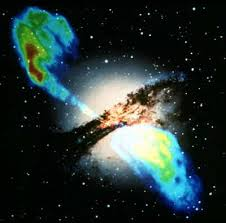
\includegraphics[scale=1.5]{agn.jpeg}
\caption{An example of a galaxy with AGN jets from radio spectrum overlaid}
\label{fig:agn}
\end{figure}

\subsection{Causes of Jets}

The causes of the emission of these kilo-parsec size jets from the centre of AGN is not fully understood, although modern theories indicate that it is related to the interaction of accretion disks in or near the event horizons of the SMBHs they surround \footnote{\cite{redjets}}. possible theories for the cause of these jets are:

\begin{itemize}
    \item The interaction of magnetic fields with the event horizon. The idea behind this theory is that magnetic fields become twisted and extremely dense and matter falls into the black hole so shortly before the event horizon, the tremendous energy that is contained in the accretion disk at that point causes the emission of twin jets out into the universe \footnote{\cite{jetcause}}
    \item frame dragging: This is an effect predicted from Einstein's general theory of relativity. The idea is that a rotating black hole, rather like a rotating cylinder in a fluid, will cause space time around the event horizon of a black hole to rotate at different rates. The interaction of the matter with this "twisted" area of space-time immediately before the event horizon has been identified as a possible cause of the emission of the jets that this project is concerned with. \footnote{\cite{framedrag, grav}}
\end{itemize}

It is possible that both of these processes \footnote{\cite{jetspaper}}, or other, yet to be described or identified causes could be responsible for the emission of these jets from AGN's. Regardless of the nature of the actual cause(s) of the emission of jets form AGN, it will almost certainly be linked to the presence and interaction of accretion disks with the SMBH that they accumulate around. An exiting development in this field, which may well yield greater insight into and possibly even resolve the mystery of the causes behind jet emmissions from AGN are observations from the aptly named even horizon telescope \footnote{\cite{eventhorizontelescope}}, which aim to obtain direct radio images of the SMBHs M87 as well as Sagitarius A, the SMBH dected at the centre of our galaxy, the milky way.



\subsection{Types of Emission}

The processes which cause the main types of radiation observed from the radio loud jets are thought to be: synchrotron, reverse-Compton scattering, and thermal bremsstrahlung\footnote{\cite{Hardcastle}}. As the HETDEX survey is in the radio frequency, this project will focus on synchrotron radiation, because of the three forms of radiation emitted from AGN, it is the only one which emits significant electromagnetic emission that can be detected at radio wavelengths. A description of the phenomena, and what the emissions can be used to infer are discussed below.

\subsubsection{Synchrotron Emission}

\begin{figure}
\centering
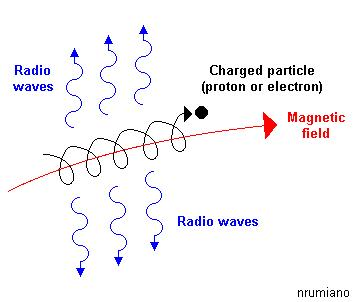
\includegraphics[scale=0.7]{synchrotron_radiation.jpg}
\caption{Illustration of synchrotron radiation}
\label{fig:sr}
\end{figure}


Any time a charged particle undergoes an acceleration, by either moving in a curved path or changing velocity linearly, it will emit radiation in the form of photons. This phenomenon is known as synchrotron radiation (not to be confused with a synchrotron which is a device which accelerates charged particles in a curved path) \footnote{\cite{synch}}. The power dissipated by these emissions is proportional to the fourth power of the speed of the charged particle and as it be expected follows and radial inverse square law for its spacial dissipation.  In a classical regime, the formula for the power radiated from a charged particle is given by Lamor's formula\footnote{\cite{lamor}}, which can be expressed as:
\begin{equation}
   P = 2Ke^2a^2/3c^3
\end{equation}
As the particles that we are dealing with are moving at relativistic speeds, the formula for emitted power becomes:
\begin{equation}
    P = 1.25\sigma cU \gamma^2
\end{equation}
where the sigma is the Thompson cross-section \footnote{\cite{Thompson}}, and the U is the energy density in the magnetic field. Dividing the energy of the synchrotron radiation by the power gives us the following formula for the time scale for energy loss:

\begin{equation}
    \tau = 3mc/4 \sigma U \gamma    
\end{equation}

This formula indicates that the rate of energy loss is proportional to the energy of the the charged particle. By considering that an individual charged charged particle (in this case an electron) has spectrum of synchrotron emission which is highly peaked at approximately:

\begin{equation}
    \gamma^2 eB/2 \pi m
\end{equation}

and combining the above with equation (3), we can infer maximum possible times since emissions, given that the strength of the magnetic field, B is known. Observed radiation however, is detected from a range of energies, to account for this we must think in terms of synchrotron energy emitted per unit volume, which is given by\footnote{\cite{Hardcastle}}

\begin{equation}
    J(\nu) = (\sqrt{3}B^3\sin(\theta)/4\pi\epsilon_0cm) \int_{E_1}^{E_2} F(x)N(E) dE
\end{equation}

where $E_1$ and $E_2$ are the minimum and maximum energies detected respectively, N(E) is electron energy distribution function and F(x), is the function which describes the spectrum of the synchrotron radiation of an individual electron given by

\begin{equation}
    F(x) = x \int_{x}^{\infty} K_{5/3} (z) dz
\end{equation}


$K_{5/3}$ is a modified Bessel function. As the value of F(x) becomes negligible when $x>1$, it is N(E) which the dominant factor in determining the observed synchrotron radiation emission spectra. As the observed emission spectra can be described by a power law:

\begin{equation}
    N(E) = N_0E^{-P}
\end{equation}

we can integrate equation (5) over electron energy and pitch angle; which is assumed to be isotropic to obtain

\begin{equation}
    J(\nu) = CN_0\nu^{-(p-1)/2}B^{p+1/2}
\end{equation}

where

\begin{equation}
    C = c(p)(e^3/\epsilon_0 c m_e)(m_e^3 c^4/e)^{-(p-1)/2}
\end{equation}
c(p) is a combination of gamma functions of order 0.05 which depend weakly on p. From equation (8), it can be seen that electron energy spectral index can be inferred from the dependence of the synchrotron radiation's luminosity on frequency. This power law dependency deviates over time so that, eventually for $ E < 1/at $:
\begin{equation}
    N(E) = N_0E^{-p} (1-Eat)^{p-2}
\end{equation}
for $E \geq 1/at$, N(E) = 0. The above equations can be used to estimate an emission time (and therefore distance), given that a value for the magnetic field strength is known. In practice this is difficult to obtain from observations. Not having a value for the magnetic field strength means that a value for the total energy density, U:
\begin{equation}
    U = \frac{B^2}{2\mu_0} + (1 + \kappa) \int_{E_1}^{E_2} EN(E)dE
\end{equation}
is also unobtainable. The $1 + \kappa$ in the above equation is a factor which accounts for the energy of non-radiating particles. If assume that the electron energy spectrum has the shape of a power law, the above integral can be solved up to the normalisation of the power law of $N_0$, and given that we have a relation between emissivity, normalisation and magnetic field strength from equation (8), we can use it to eliminate B from equation (11) and get a value for minimum field strength. If we assume $\kappa = 0$ then this implies that the magnetic field strength corresponds to the energy being in equipartition between the field and the electrons. Given that there are so many assumptions in these calculations of field strength, it is impossible to state how accurate the times and distances obtained from these calculations are.

A final feature to note about synchrotron emission is that it is strongly polarised. The fractional polarisation can be obtained by integration the polarised emissivity function for a single electron, G(x) over electron energy and dividing it by the total emissivity:
\begin{equation}
    \Pi = \frac{\int G(x)N(E)dE}{\int F(x)N(E)dE}
\end{equation}
Fractional polarisation is not dependent on magnetic field strength. It only depends on the nature of the electron energy spectrum. In a region where the magnetic field strength is uniform, the direction of the electric field would be perpendicular to the direction of the magnetic field. However, in a realistic field surrounding an accretion disk, the field would be far more complex and effects such as Faraday rotation would distort the emitted particles further. An estimate of the rotation angle, $\phi$ can be obtained if we were to assume that that the thermal electrons are external to the radio source:
\begin{equation}
    \phi = c^2\kappa/\nu^2 \int_{s}^{0} nBds
\end{equation}
$\kappa$ here is a constant and the integral is evaluated along the line of sight to the source, implying that the rotation angle depends on the wavelength squared. Once again this ideal case may well be to simplistic to account for other effects in observed sources.

\subsection{Aims and Objectives}

As previously stated the main aim of the project is to determine a method to automate the detection of the relevant AGN jets. The two main parameters that would need to be manipulated, to find the right cut off between correctly identifying as many relevant sources as possible, while avoiding false positives are: size and luminosity. Another objective to ascertain if there is a selection bias in the data that we have selected, and if so investigate if there is a certain class of galaxy that is preferentially selected by the selection criteria. \newpage

\section{Radio Astronomy}

\begin{figure}
    \centering
    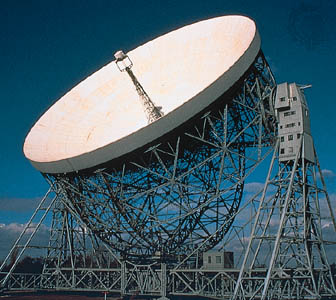
\includegraphics{Lovell Telescope.jpg}
    \caption{An example of a Radio Telescope, known as the Lovell Telescope, based in Cheshire, England}
    \label{fig:Lovell}
\end{figure}

This section will discuss the physics behind radio astronomy, how it is done and what uses it has. The fact that it especially useful in identifying and studying AGN jets and their possible causes has been already been discussed in the section above.

\subsection{Utility}

\begin{figure}
\centering
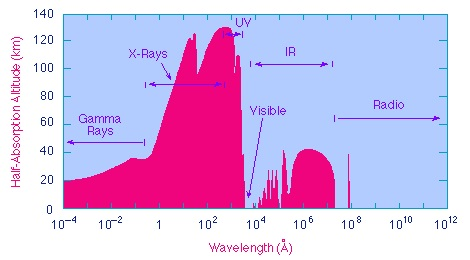
\includegraphics{atmos_windows.jpg}
\caption{absorption of electromagnetic radiation from space by the Earth's atmosphere}
\label{fig:atmosphere}
\end{figure}

As can be seen from the diagram above, the atmosphere of the Earth absorbs all or most of the incident electromagnetic radiation on it apart from into relatively narrow channels (when compared to the entirety of the electromagnetic spectrum). The penetrating wavelength correspond to visible light (which is rather obvious, as else we would observe nothing but a blank, black canvas when observing the heavens at night) and at certain frequencies of radio waves. This therefore makes those radio waves of great interest to astronomers. An additional property, not immediately obvious from the figure above is that radio wavelength radiation can often penetrate the dust and gas present in the space between the source of their emissions and the point of detection. This means that radio astronomy offers a more complete view of the universe, giving scientists the ability to identify and study objects which emit radio wavelength radiation that would not be possible at other wavelengths. \footnote{\cite{radiobook, eradio, fradio}} The methods that are used to collect and interpret the radiation are discussed below.


\subsection{Method}

There are two fundamental components of any radio telescope: 

\begin{itemize}

    \item the antenna (see the large white disk in figure 3.): The antenna acts as a collecting bowl for the incident radiation, and tends to of a parabolic shape, so that the collected radiation can be directed to the sub reflector (the small "blob" in the centre of the dish, on top of the pole). Due to the fact that radio signals from space tend to be extremely weak; antenna sizes tend to be very large. The factors mentioned above mean that radio telescopes are often located in remote locations, in order to shield them from the relatively much stronger radio signals generated from Earth based technology. Although extra terrestrial radio signals can be detects from many points on the surface of the earth, the best quality of signal is achieved in arid, high altitude conditions; therefore modern, telescopes are often found in locations that are both high and dry.
    
    \item The radiometer: is a device used to measure the intensity of the incoming radiation.
    
\end{itemize}

In modern radio telescopes, the signal processed by the radiometer would then be transmitted digitally to a computer to be analysed \footnote{This is normally done by performing a Fourier transform on the incident signal and the displaying it using specialist software \cite{radiobook}} and finally the output would be generated and stored ready to be viewed by astronomers (see figure 5 below). Modern radio telescopes are often actually a large collection of individual telescopes which are combined to produce a more accurate or wider range of image.

\begin{figure}
    \centering
    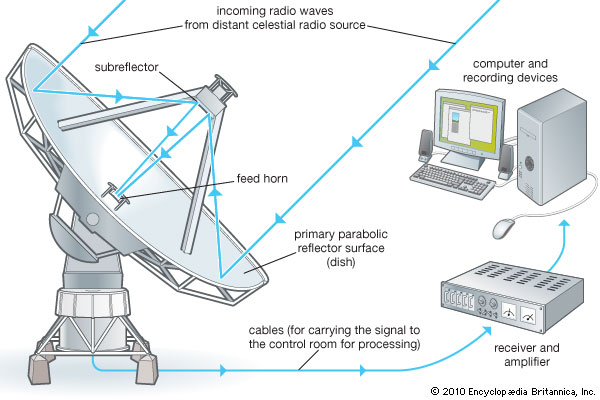
\includegraphics[scale = 0.5]{radio_works.jpg}
    \caption{Schematic diagram of the workings of a typical modern radio telescope}
    \label{fig:radio work}
\end{figure}

While radio telescope have a wide range of applications in astronomy, we will focus our concern on those telescopes which are used to study the sky and detect AGN and their associated jets. The telescope that is the most advanced currently available is known as LOFAR and is discussed below.

\subsection{LOFAR}
The Low Frequency Array (LOFAR) \footnote{\cite{lofarweb,lofararticle,lofaruk}} is currently (as of February 2017), the worlds most sensitive low frequency radio telescope, for a wide range of frequencies.\footnote{For a narrow range of frequencies the Event Horizon telescope (see \cite{eventhorizontelescope}) is more sensitive still. As this telescope is composed of several other detectors around the globe, rather than detectors that were purpose built, and is used for very different purposes (LOFAR is used to scan the entire northern sky, giving us a complete radio picture, whereas Event Horizon is designed to focus on small range of very specific locations. It is therefore difficult to compare the two.} Based largely in the Netherlands, with some of the detectors present in Germany, Great Britain, France, and Sweden. As it is located entirely in the northern hemisphere, it can only be used to generate radio maps of the northern sky. It has already been used extensively to generate a number of surveys of the sky, some of which are complete. Some of the survey which have been completed are discussed below, as well as an element of LOFAR Two-metre Sky Survey, known as the HEDTEX (see HETDEX subsection for more information) survey which, while not a complete survey of the northern sky (the version used in this research covers an area of 100 degrees squared), is the most sensitive survey that we currently have.


\subsection{Bo{\"o}tes}
The Bo{\"o}tes \footnote{\cite{bootes}} sky survey is a wide area (it covers 19 degrees of the sky) and high resolution radio map of the sky. Initial observations were made in 2014, with a published introduction to the survey appearing in 2016. While many of the techniques developed and used in preparing and cleaning the final mosaic image were useful in future surveys, relative to the HETDEX survey, the image suffered from artefact contamination, chiefly due to calibration errors. (see mosaic image).

\begin{figure}
    \centering
    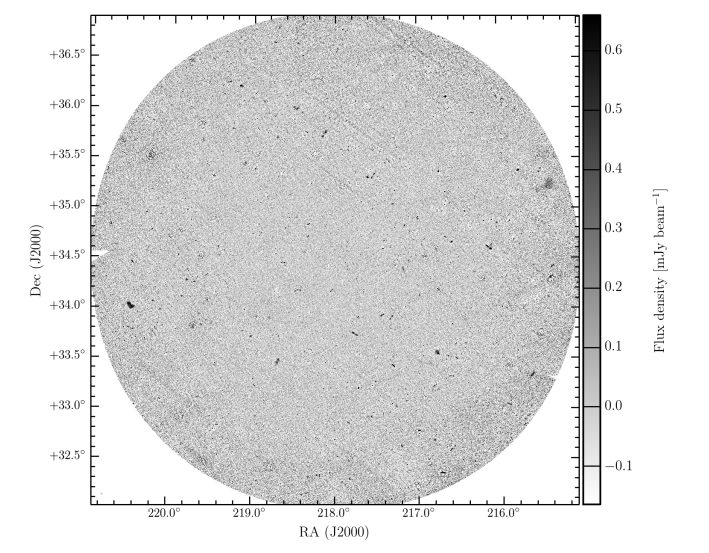
\includegraphics[scale = 0.5]{bootes.png}
    \caption{The complete survey of the Bo{\"o}tes field in one image}
\end{figure}

\subsection{Herschel}
Also known as the Herschel-ATLAS survey of the north galactic pole field\footnote{\cite{hatlas}}. It is the most recent complete low-frequency, high-bandwidth which covers approximately 142 degrees of the northern sky. While the Herschel survey produces a map which is both more detailed and cleaner, i.e. with fewer artefacts, issues still remain with the uniformity of the image and consistency of for all areas of the sky.

\subsection{HETDEX}

The Hobby-Eberly Dark Energy Experiment, (HETDEX) is a visual survey concerned with the investigation of dark energy \footnote{\cite{HETDEX}}. The LOFAR Two-metre Sky Survey (LoTSS), which aims to eventually be the most sensitive complete radio survey of the northern sky, currently has active data collected in the same section of the northern sky as HETDEX proper. The data from the HETDEX \footnote{\cite{lofar2}} survey of the northern sky is the basis for the research conducted in this dissertation. It was selected due to the project supervisors knowledge of the survey, the fact that all of the data was readily accessible on the University of Hertfordshire's supercomputer, as well the fact that was at the time, the most sensitive survey of the northern sky ever done at radio frequencies. For the sake of clarity, in future when HETDEX will be referred to, that will mean the LoTSS survey of the section of the sky covered by HETDEX. Pybdsm has identified approximately 85,000 sources in the HETDEX survey, many of which are of exceptional clarity. While this is a great achievement, a sub selection of those sources would need to be made, in order for any meaningful analysis to be possible. The next section discusses how this selection was achieved.
\newpage

\section{Selecting sources}
As previously mentioned the total number of sources in the survey was far to high too be analysed individually. (see diagram) Therefore a subset of this data selected, yielding a suitable number and type of sources which could be used further in our optical analysis. The types of sources sought after in the selection would be as clear, large and bright as possible. The reasons why behind the selection criteria, the final criteria themselves and the tools as well as the method used are all discussed below.

\begin{figure}
    \centering
    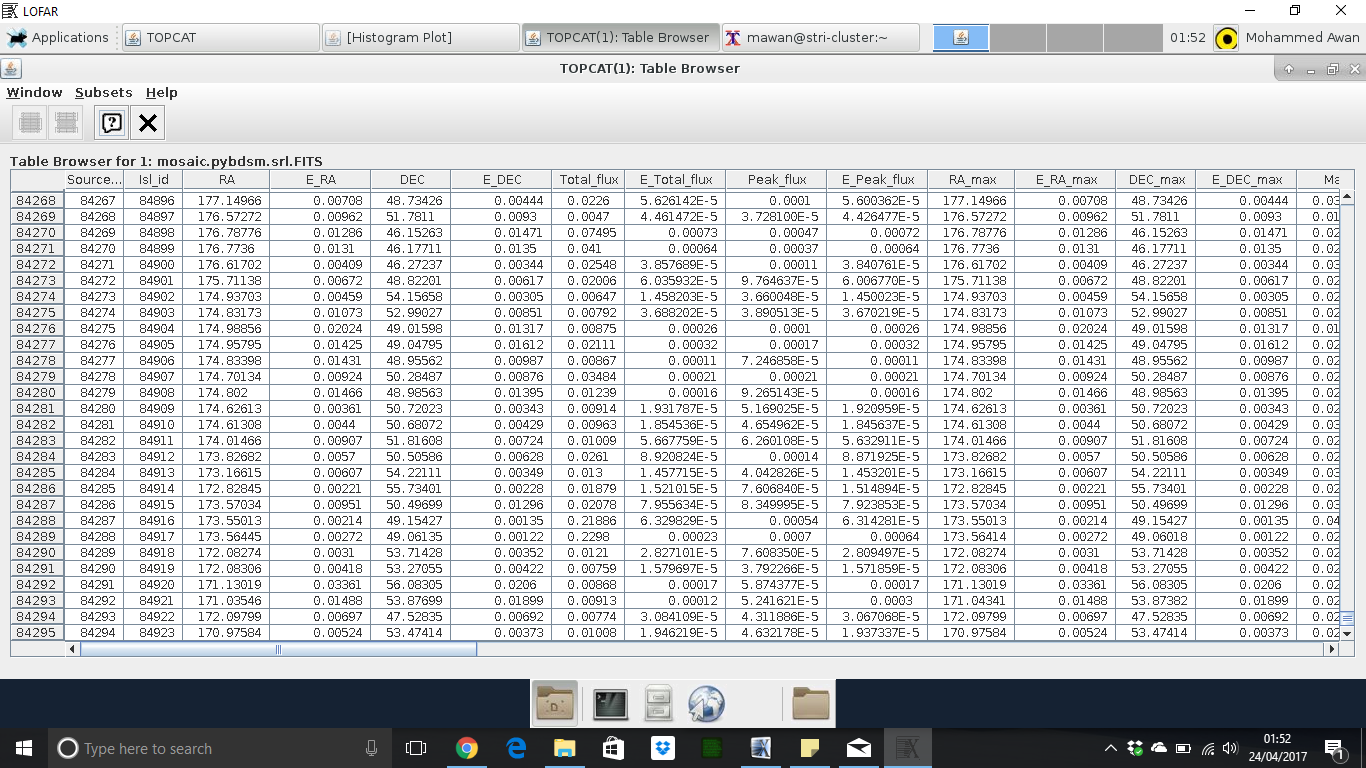
\includegraphics[scale = 0.3]{mdata.png}
    \caption{screenshot of the fits file for HETDEX loaded into topcat, note the number in the bottom left hand corner: 84925; this is the total number of sources in identified in the survey!}
\end{figure}

\subsection{objective}
The first step in obtaining the data necessary for the analysis and future use in automatic detection, after gaining some familiarity with the tools used to access the data, was to gather a suitable selection of sources that could be linked to visual sources. The suggested target size was approximately 250 sources.

\subsection{tools}
The entirety of the data from the HETDEX survey that is stored on the University of Hertfordshire's supercomputer is accessible via the use of a virtual machine (the specific program used to call the terminal is called X2goclient) on a Debian Linux distribution. Other programs that were used in the selection of the sources is below:

\begin{itemize}
    \item X2goclient: This is the application that was used to remotely access the HETDEX data that is stored on the University of Hertfordshire STRI cluster server. It is a remote desktop program allowing the user (known as the client) to access another computer (known as the server) remotely. For this work, the server was accessed via a Linux PC based in the PAM school in the University of Hertfordshire as well as the author's personal windows 10 based laptop.
    
    \begin{figure}
        \centering
        \includegraphics[scale = 0.3]{x2goterminal.png}
        \caption{Screenshot of x2go terminal on Windows 10 o/s}
        \label{fig:x2go}    
    \end{figure}
    
    \item LOFAR Linux virtual machine: The remote server actually used to access the HETDEX array data, to store selected sources as fits files, as well as images generated for optical identification. Practically all of the actual work behind the project was done on this server. (see figure 7 and 8)
    
    \begin{figure}
        \centering
        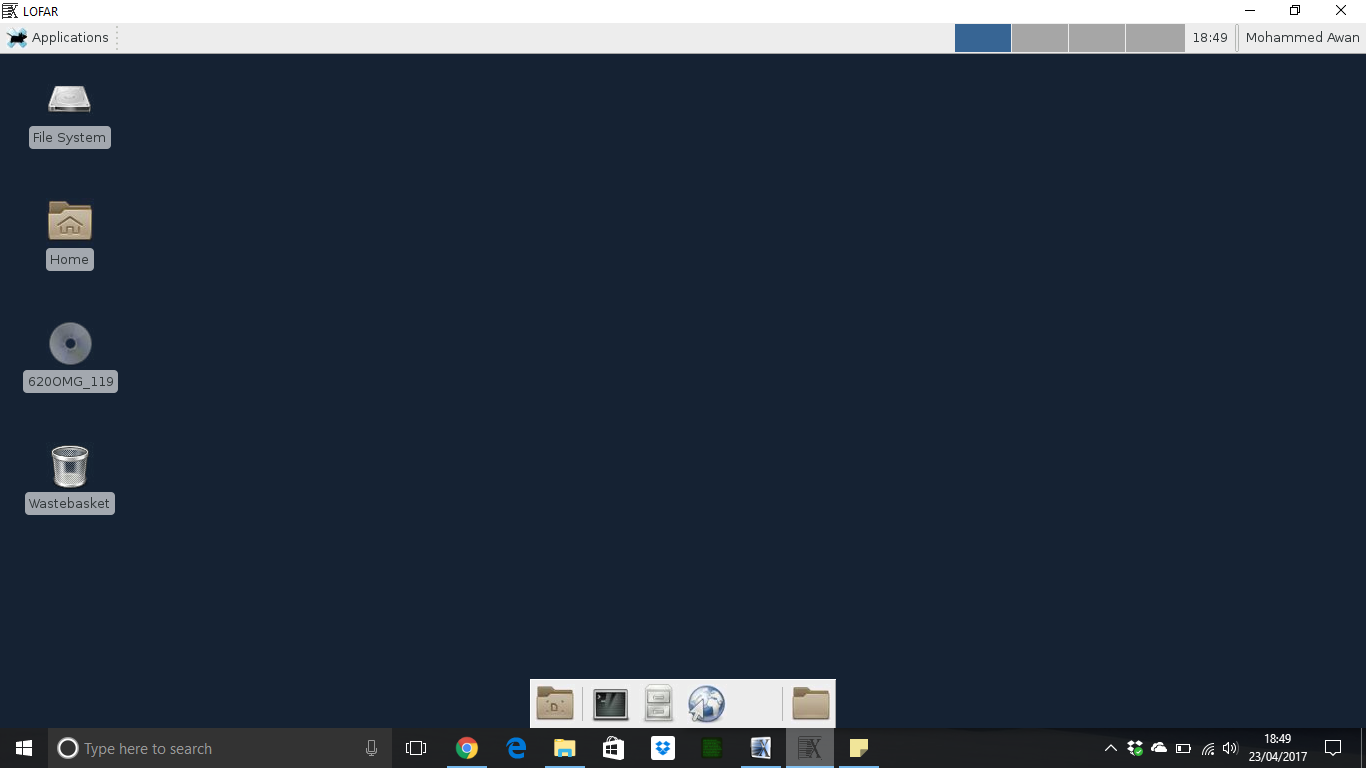
\includegraphics[scale = 0.3]{LOFARclient.png}
        \caption{Image of the LOFAR Linux server when initialised}
    \end{figure}

    \begin{figure}
        \centering
        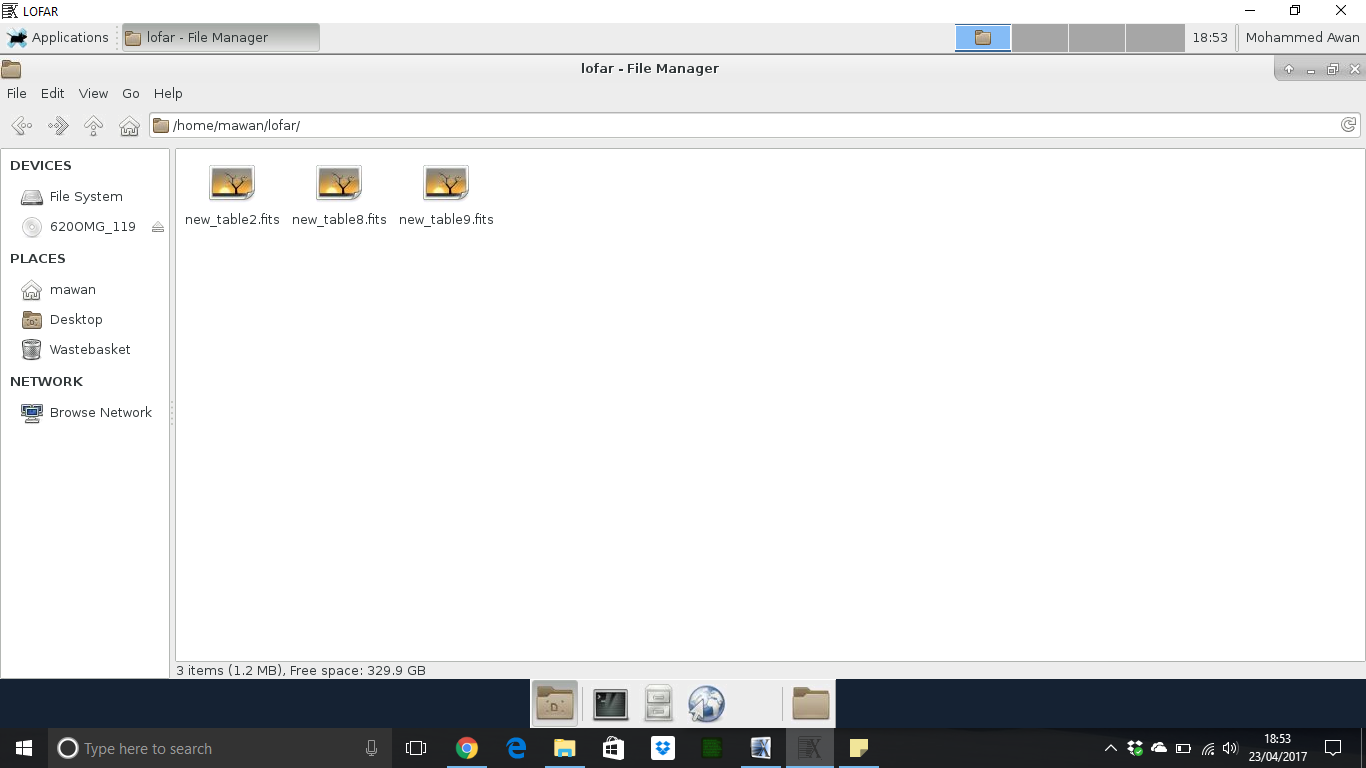
\includegraphics[scale = 0.3]{selectiondataexample.png}
        \caption{Image of directory where the selections of total data was stored (location on the server was /home/mawan/lofar}
    \end{figure}
    
    \item Xterminal: One of the many programs that can be used to access the Linux terminal (a command line processing environment) that can be used to create folders, store data in them, launch the programs below and also act as an environment for our primary programming language used in this project namely, python\footnote{\cite{python}}. Almost all of the commands to run scripts created by others or create selections using the python programming language or even to launch applications were done here. (see figure 9)
    
    \begin{figure}
        \centering
        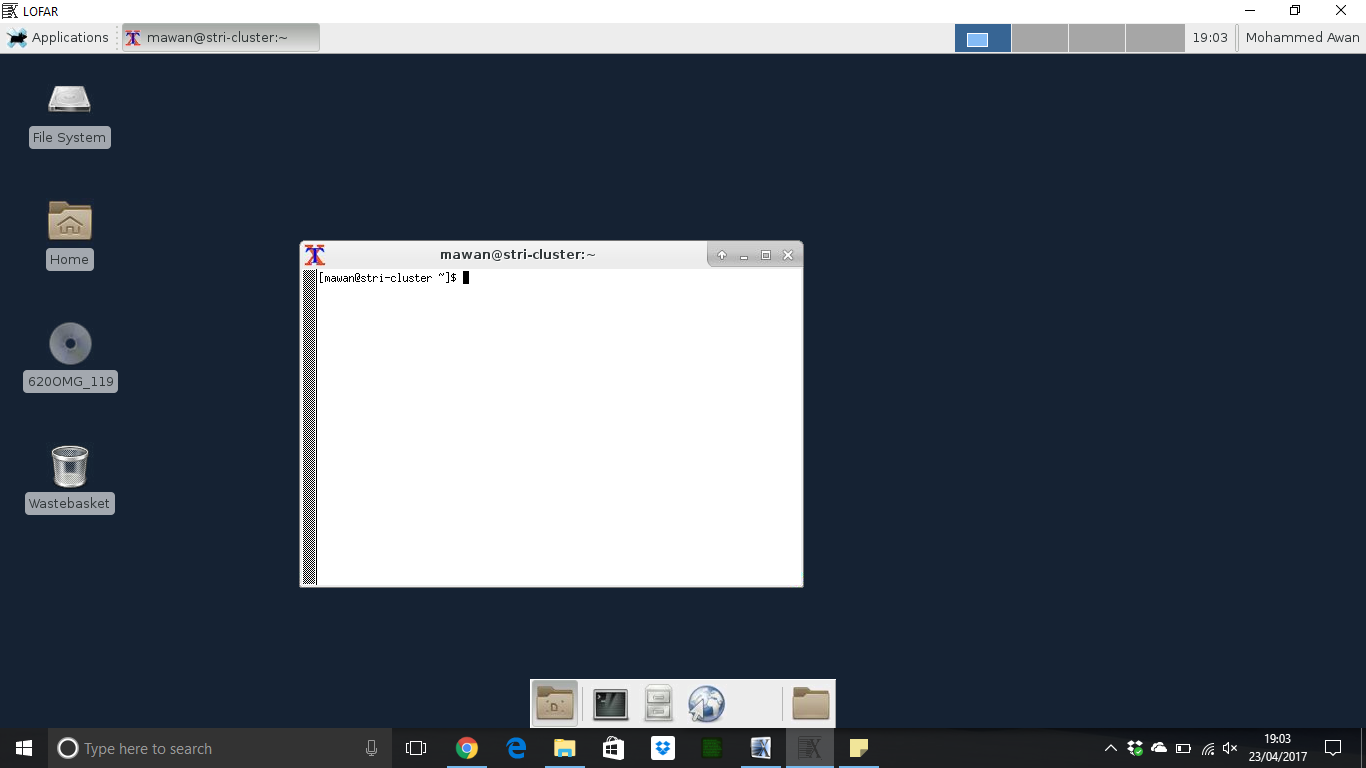
\includegraphics[scale = 0.3]{xterminal.png}
        \caption{X terminal when initialised}
    \end{figure}
    
    \item Topcat: used to load the databases (which were in the form of fits files) into for the purposes of analysis and, chiefly so that they could be used by ds9. It can also be used rather like Microsoft's excel, to view the databases directly and also generate plots (see figure 11 for image and analysis section for examples). code used to open application in the terminal was \texttt{/soft/topcat/topcat.}
    
    \begin{figure}
        \centering
        \includegraphics[scale = 0.3]{topcat.png}
        \caption{Image of topcat program (before any tables are loaded)}
    \end{figure}
    
    \item pybdsm: A program used to identify radio sources in the HETDEX survey (by use of gaussian methods). The images would then be displayed in ds9 with bright green rings surrounding them.
    
    \item ds9: The program that would display the radio images of the selected images in conjunction with pybdsm.
    
    \begin{figure}
        \centering
        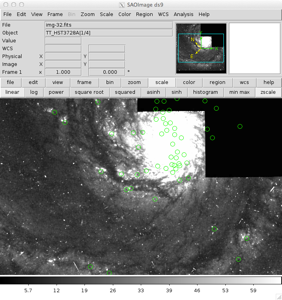
\includegraphics{ds9.png}
        \caption{An example of an image displayed in ds9 with identified sources circled}
    \end{figure}
    
    \item ipython: this was the "in-terminal" environment used to execute python code. The source selection was done using this environment.
    
    \begin{figure}
        \centering
        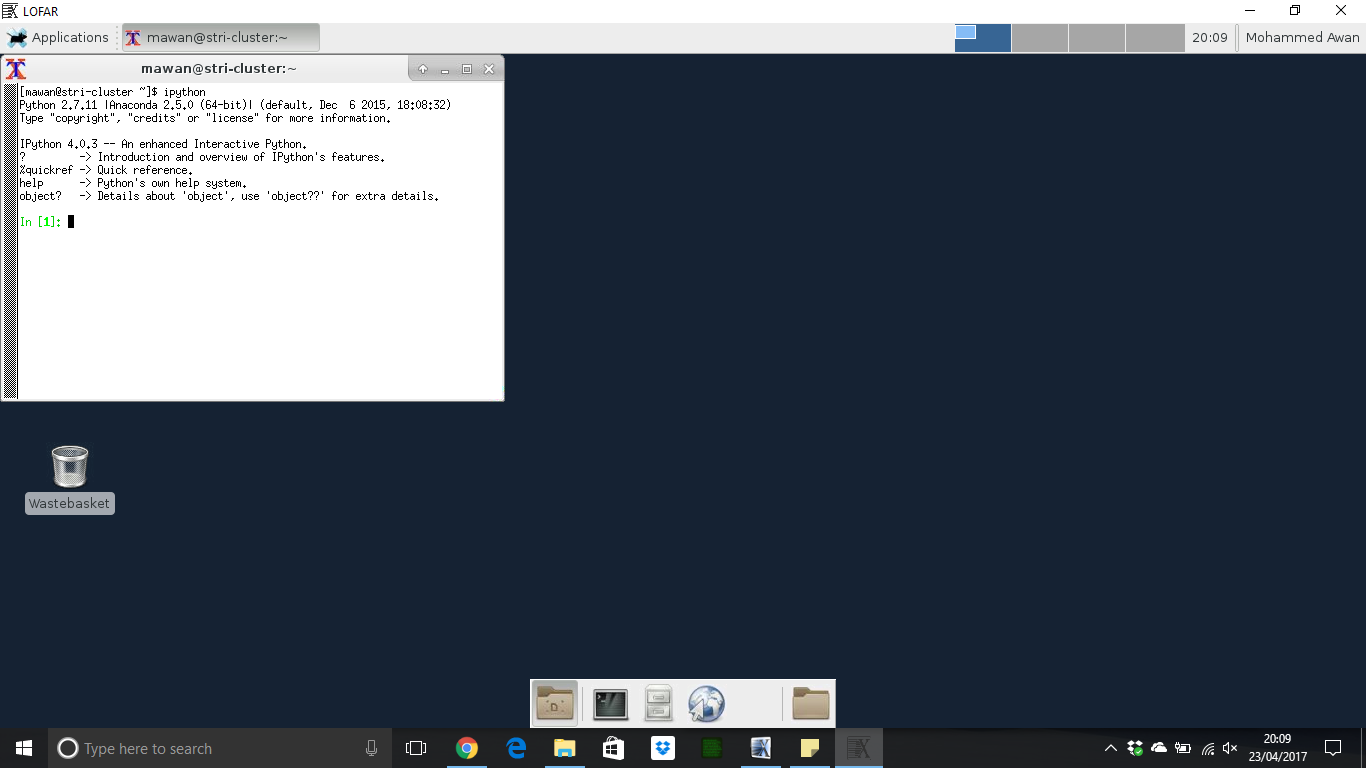
\includegraphics[scale = 0.3]{ipython.png}
        \caption{image of ipython environment initalised within xterminal}
    \end{figure}
    
    \item python: The python programming language, in particular the astropy and numpy libraries were called upon extensively in the project in order to process the data. Many pre-prepared scripts were used in order to assist in selection and later in the optical identification of the sources; where the radio images from hetdex were overlaid on visual frequency images from the panstarrs library. This included external programs written in python, such as pybdsm (which was specifically developed for source identification in radio astronomy from the lofar array) as well as specific scripts written for this project by its' supervisor.
\end{itemize}

A description of how the selection was performed is below.

\subsection{description of method}

\begin{itemize}
    \item Firstly, the x2go client was initialised and the lofar data was accessed via the terminal
    \item Once the terminal was initialised, topcat was run using the command: /soft/topcat/topcat
    \item once topcat initialised, the pybdsm.srl.fits database was opened in it.
    \item the selection process could now begin by loading python using, the ipython environment. This was done by selecting a subset (taking a slice from the main tables to use python terminology) of the main data on criteria to be investigated. After consultation with my supervisor it was decided that the apparent brightness of the identified source (called 'Total{\_}flux' in the main fits table) and the size of the object (known as 'Maj' \footnote{'Maj' actually stands major-axis. This is because the identified images are encircled by an ellipsis, or which maj is the major axis.})
    \item the selection was done in ipython by reading the table into the ipython terminal and then selecting a sample of the data (on the basis of logical constraints on maximum/minimum values of apparent brightness and size) to be saved into a new suitable (in fact the name newTablei was used in practice, where i stands for the current iteration of the table), after changing into the relevant directory and loading ipython the following commands were used in ipython itself:
        
    \item import astropy.table
    \item import numpy
    \item from astropy.table import Table
    \item t = Table.read('mosaic.pybdsm.srl.fits')
    \item new{\_t}able9\footnote{as explained above this instruction was actually preceded by 8 other groups of similar tables which were generated, printed, saved and then visually inspected in ds9 after being loaded in topcat, for the sake of brevity the code of all of these previous iterations is omitted} = t[(t['Total{\_}flux'] $>$ 0.05) {\&} (t['Maj'] $>$ 35/3600.)]
    \item print new{\_}table9 (see diagram below)
    \begin{figure}
        \centering
        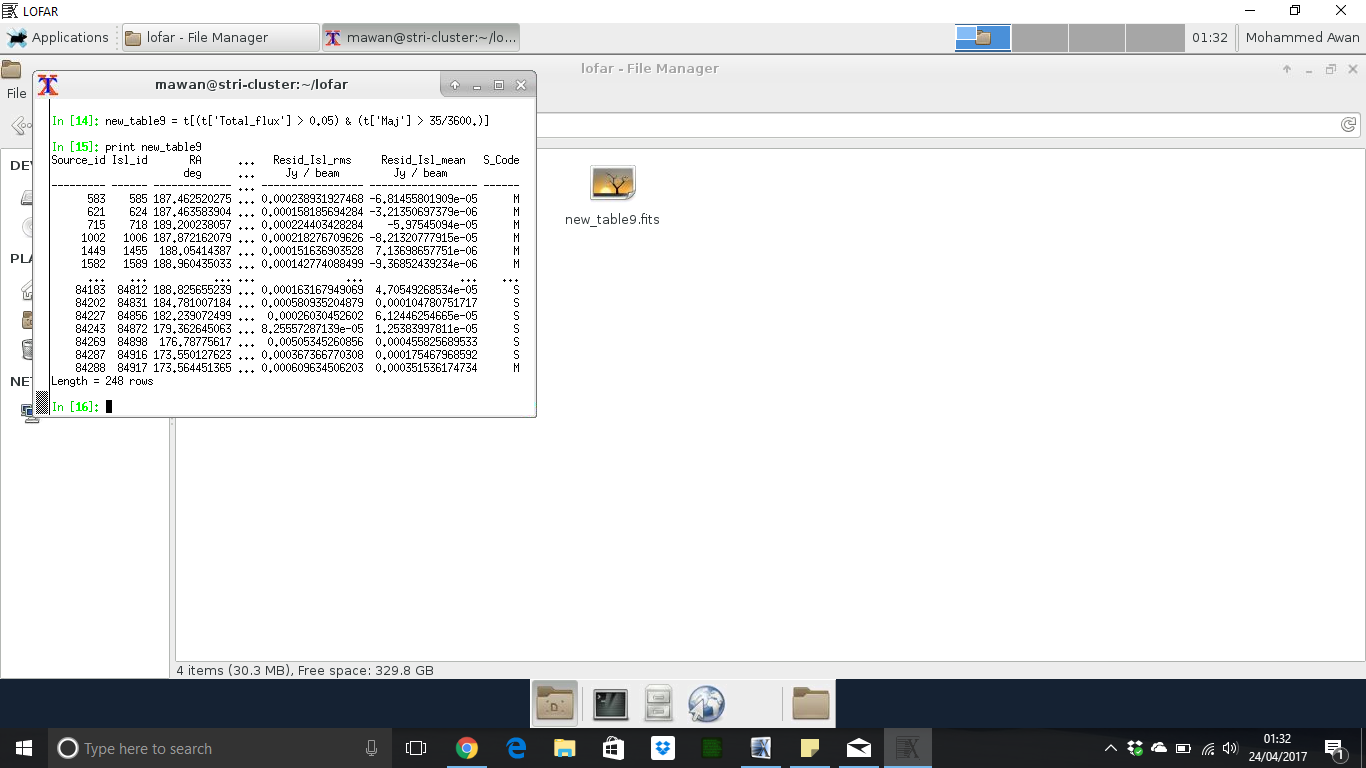
\includegraphics[scale = 0.3]{newtable9.png}
        \caption{screen shot of printed table in ipython running in xterminal. note number of rows corresponds to total number of sources in the selection}
    \end{figure}
    \item Once the selection was created, the data was then checked by loading it into the ipython environment (a truncated selection was displayed if that table was too large)
    \item the new table could then be saved 
    \item And then loaded into topcat
    \item And then finally loaded into ds9, which would display the obtained images with a green circle surrounding them
    \item the quality of the data could then be assessed
    \item Once a suitable selection was found, the data could be used for the purposes of optical identification
\end{itemize}

\subsection{causes of false positives}

\subsubsection{artefacts}
Artefacts are distortions in the image which are not caused the radio signals themselves. Often these are due to calibration errors. As the maximum resolution of a radio telescope is given by:
\begin{equation}
    \theta = \frac{\lambda}{d}
\end{equation}
where theta is maximum angular size of an object that can be resolved, lambda is the wavelength of the incident radiation and d is the diameter of the aperture, this clearly sets a rather poor baseline for aperture resolving power, due to the large wavelengths of radio waves, especially when compared to optical detection. Interference effects and electronic feedback all contribute towards the "noise" which manifest as artefacts in the final radio image.

\subsubsection{natural sources}
Not all sources in the selection would be the lobes of the AGN jets. A close galaxy with an AGN could cause false positives, as well as other AGN which are sufficiently large and bright to meet the selection criteria, such as quasars. it is also possible that an undeviated jet which is extending toward us head on, could trigger an image which would not be easily identifiable as a double lobe source.

\section{Optical Identification}
Once the sample selection was prepared, the task of optically identifying which images in the selection had equivalent sources that were observed in the visual frequencies observable by the human eye. The images for this purpose were obtained from the PAN-STARRS\footnote{\cite{panstarrs}} survey.

\subsection{method}

\begin{itemize}
    \item Firstly the table of the new selection, i.e. new{\_}table9.fits was moved to directory that was created to store the images that would be generated for optical identification. This was done by inputting the command texttt{mkdir /data/lofar/mawan} into the terminal.
    \item The PAN-STARRS images for the selection were then downloaded into the directory above, in order to processed via a python script ready for the optical identification. This was done by the following command: texttt{python /data/lofar/mjh/hetdex{\_}v2/get{\_}panstarrs{\_}file.py new{\_}table9.fits}
    \item This created a file called panstarrs-list.txt, which associates the radio and optical images
    \item After this the relevant python libraries were downloaded into the directory and then the script was then run to display the radio-optical overlays for each source, with the radio sources appearing as contours on top of the optical source with the following commands:\\
    setenv PATH /soft/Montage{\_}v3.3/bin:{\$}PATH\\
    python /data/lofar/mjh/hetdex{\_}v2/opt{\_}id{\_}hetdex.py new{\_}table.fits\footnote{the script opt{\_}id{\_}hetdex.py was created by Prof M J Hardcastle and has been omitted for the sake of brevity}
    \item This loaded an environment in the LOFAR Linux server where a terminal would output code and load a separate window with the overlaid images. Correct images had their coordinates logged via a click and images which were rejected (see below for reasons and examples of each case) were logged via pressing the return button.
\end{itemize}

\subsection{correct images}
If an image had a clear optical source, preferably in the middle of two clearly identifiable lobes, it met the criteria for being accepted into the final data set. Slightly over half the sources were suitable after being viewed optically. Some examples of correctly identified sources are below (see captions for details):

\begin{figure}
    \centering
    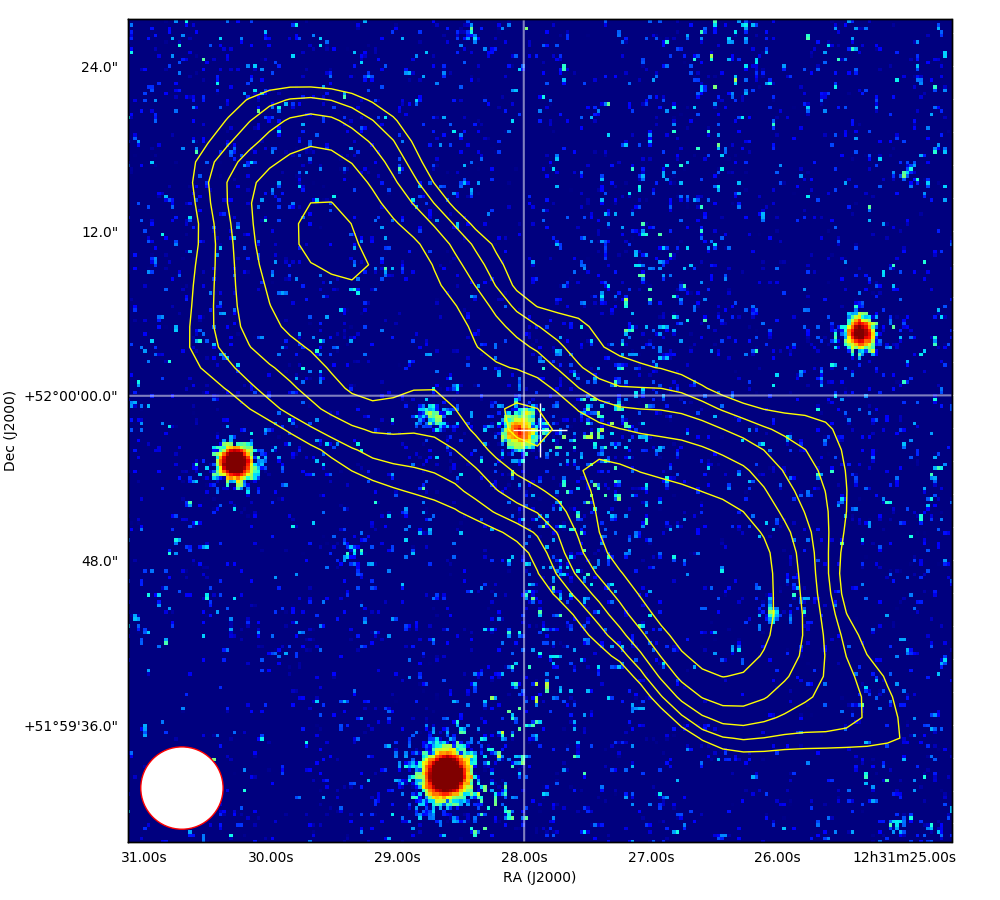
\includegraphics[scale = 0.5]{nice1.png}
    \caption{As clear as can be hoped for. The coloured blob is an optically detected galaxy sandwiched perfectly between the dual lobes}
\end{figure}

\begin{figure}
    \centering
    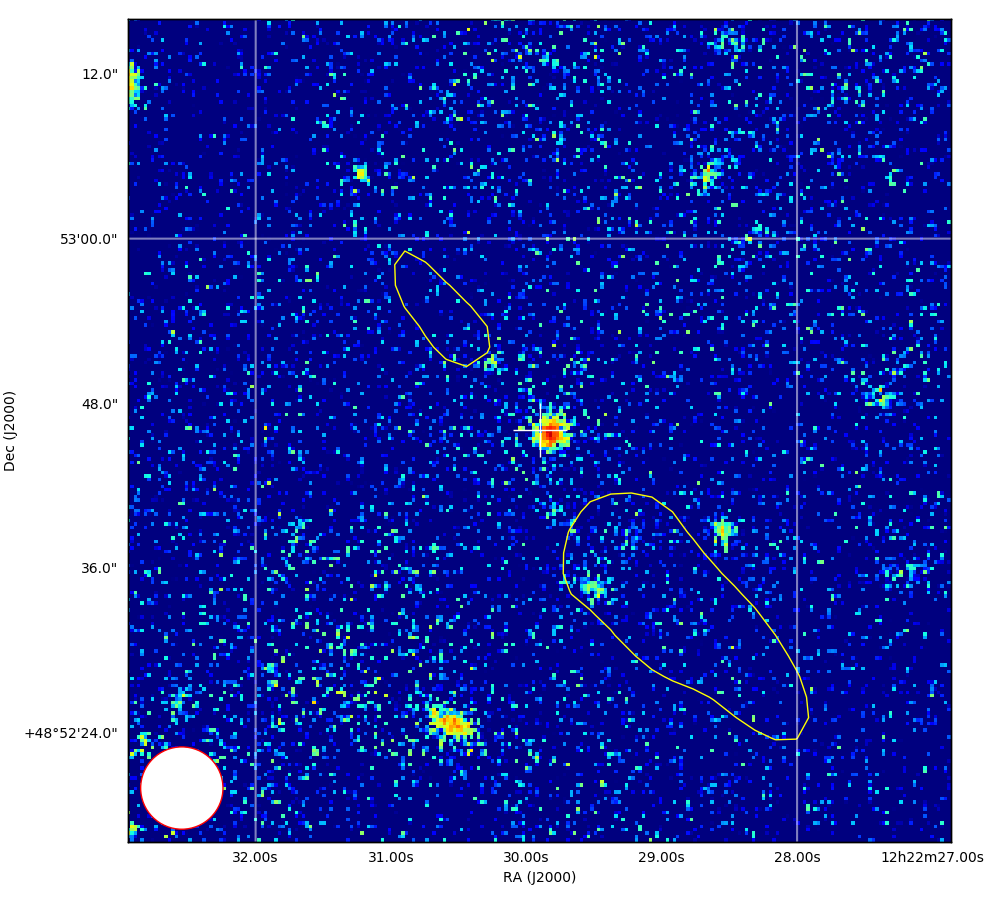
\includegraphics[scale = 0.5]{nice2.png}
    \caption{See figure above, another textbook image}
\end{figure}

\begin{figure}
    \centering
    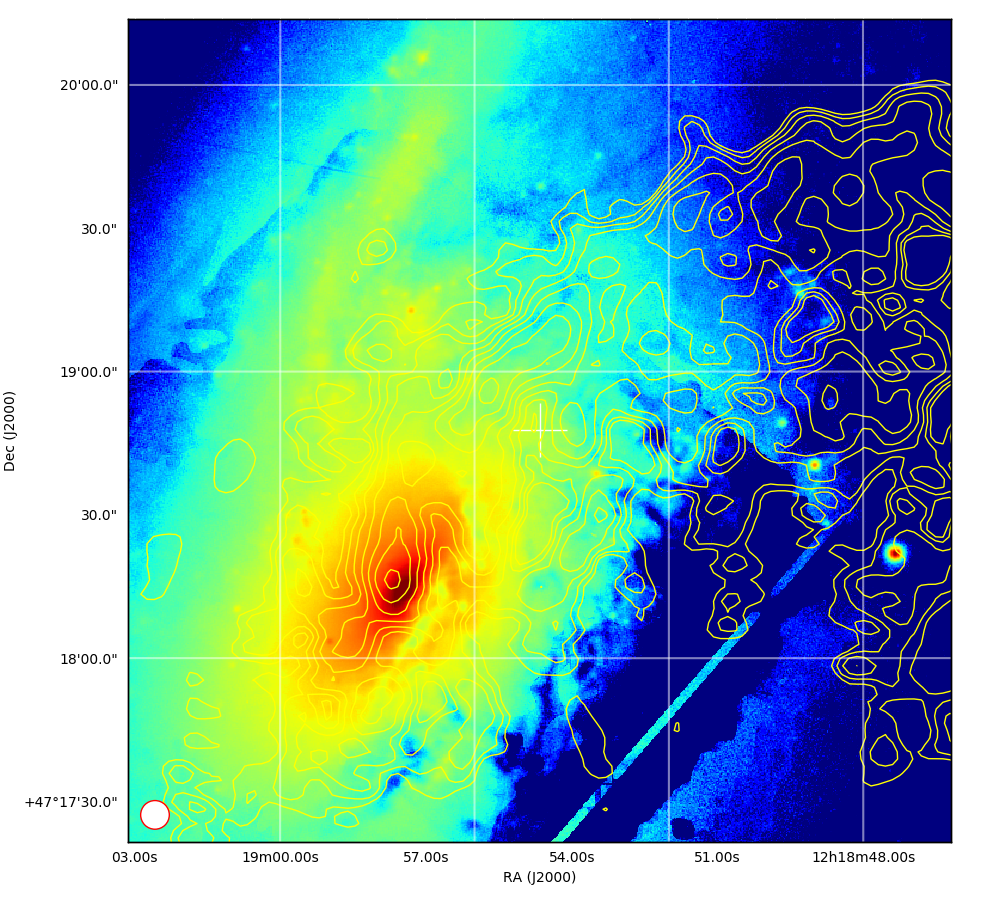
\includegraphics[scale = 0.5]{nice3.png}
    \caption{although the image is extremely bright, it is clear that the radio contours are overlaid far too congruently to preclude coincidence}
\end{figure}

\subsection{rejected images}

There are several reasons which could cause images to be rejected, see the images below and refer to their captions for further clarification:

\begin{figure}
    \centering
    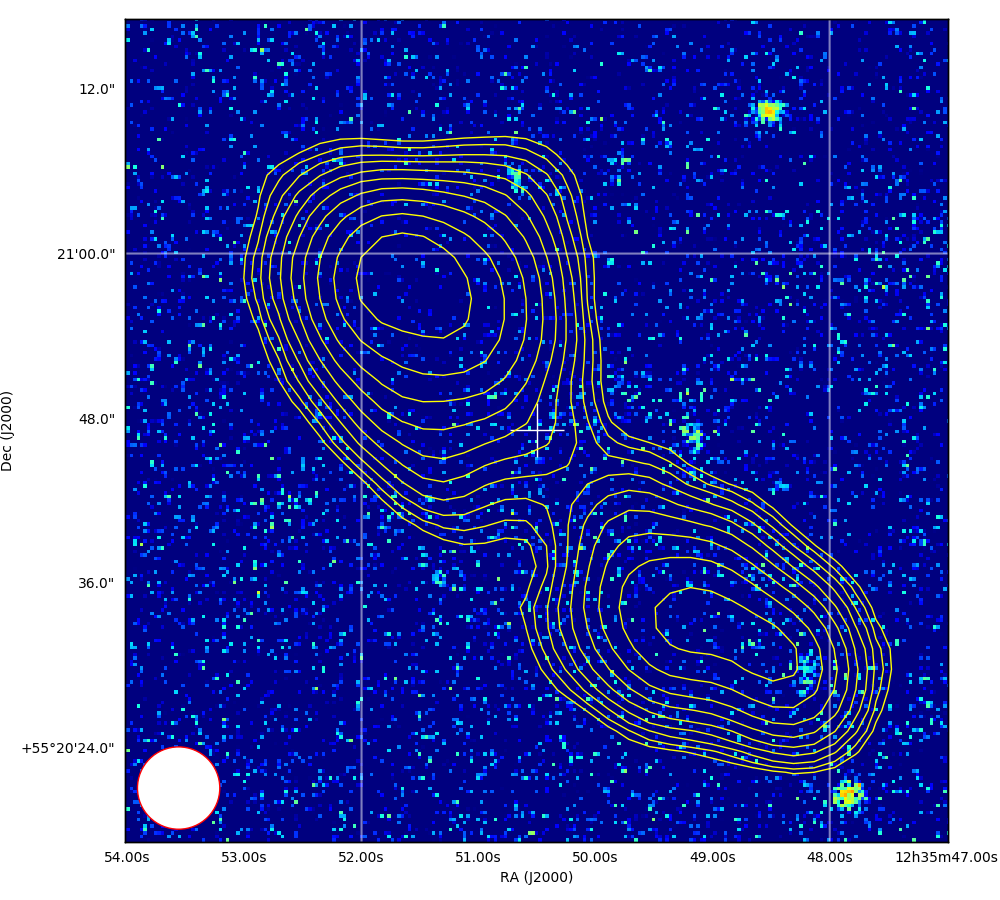
\includegraphics[scale = 0.5]{bad1.png}
    \caption{ no optical correlation is present at all}
\end{figure}

\begin{figure}
    \centering
    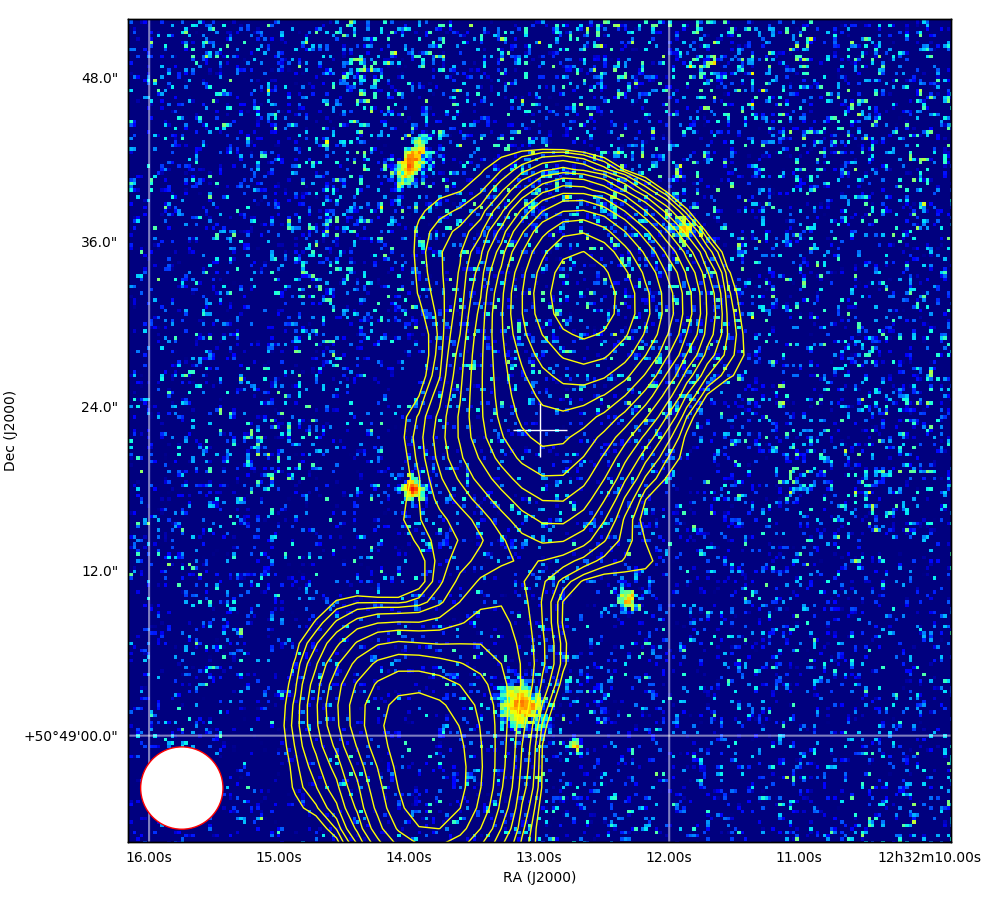
\includegraphics[scale = 0.5]{bad2.png}
    \caption{optical sources are present in the overlaid image, however there is no obvious correlation between them and the radio contours}
\end{figure}

\begin{figure}
    \centering
    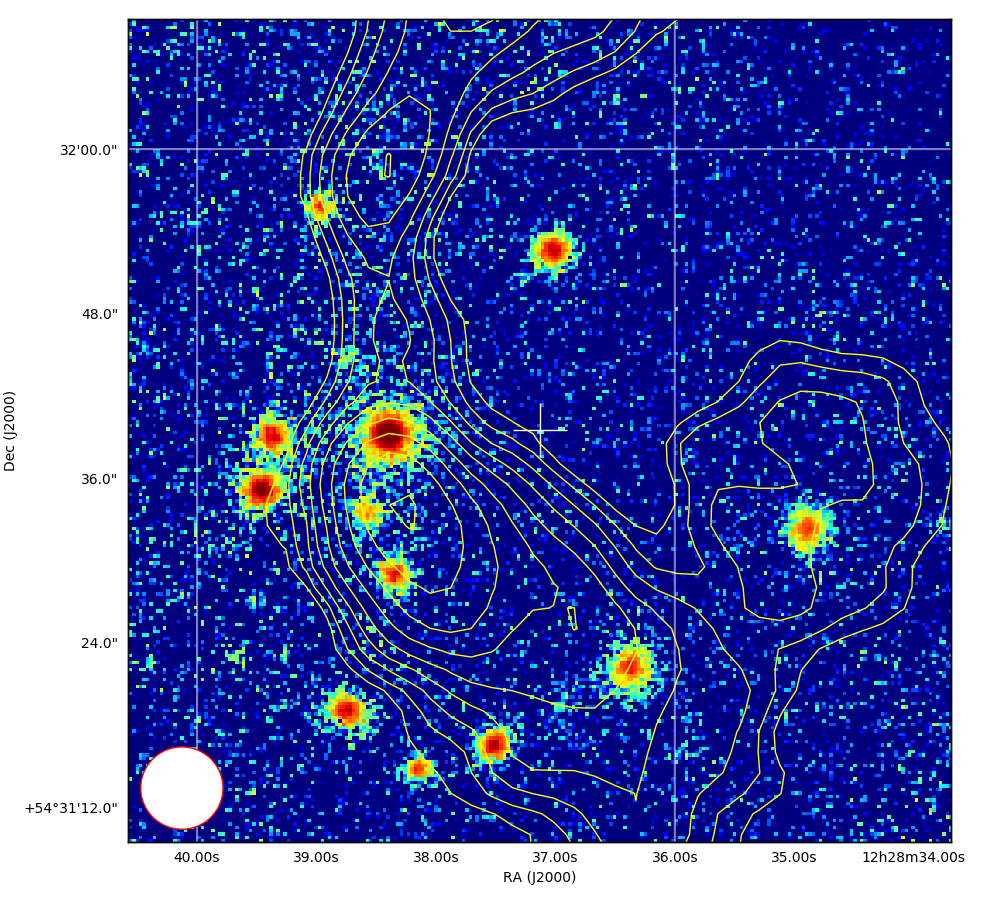
\includegraphics[scale = 0.5]{bad3.png}
    \caption{there are two many optical sources near the possible origin of the radio contours, precluding a clear identification}
\end{figure}

\begin{figure}
    \centering
    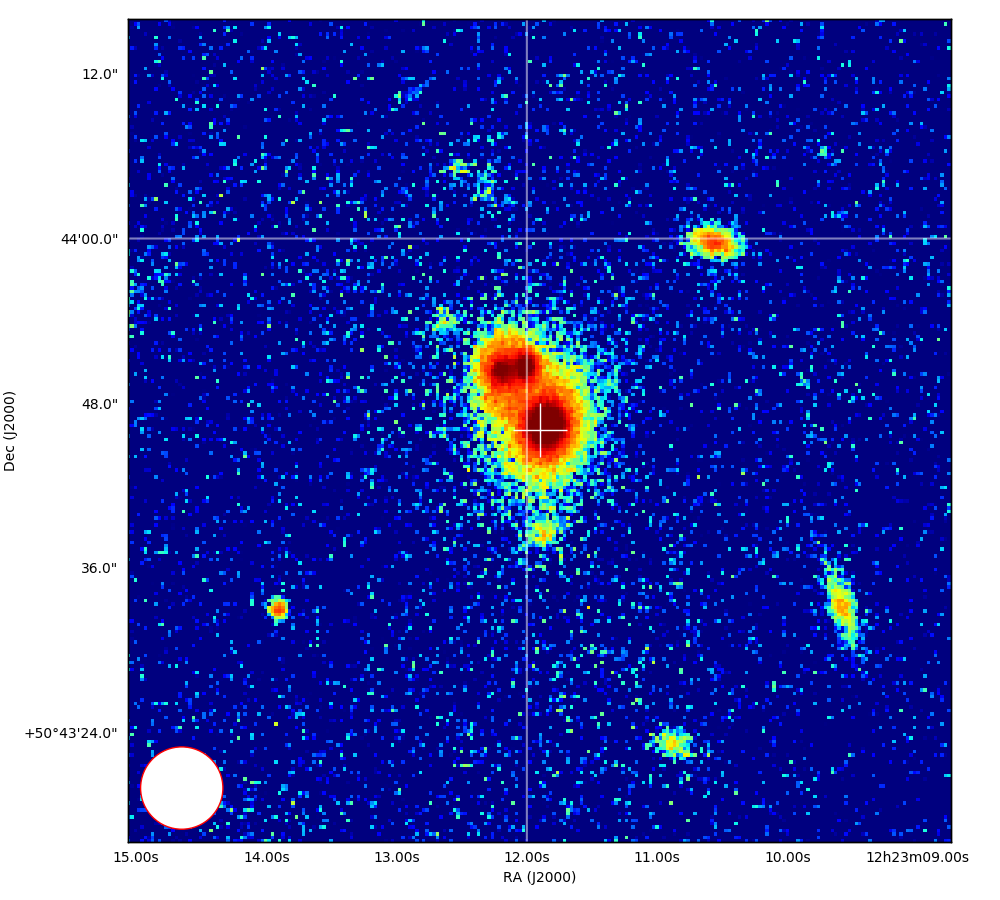
\includegraphics[scale = 0.5]{bad4.png}
    \caption{there are two issues here: an pair of colliding galaxies as opposed to one clear radio loud galaxy and the lack of any visible radio contours}
\end{figure}

\subsection{comments}
Hundreds of images were processed in preparing the final data set for analysis of underlying biases. The identification of viable sources is hardly an exact science, and a combination of interacting factors can cause an image to useful or not as the case may be. In future endeavours to automate the process, this would be a major hurdle and would require a machine with coded with some sophisticated algorithms to do the task efficiently. The job of the human interpreter however could be greatly assisted by machine processing of mass images by even relatively simple rules, for example, all images with no optical and/or radio signals would be automatically rejected. This is a rich area that would certainly justify any preliminary attempts to establish viability.
\newpage

\section{Analysis}
The final stage of the project was analysing the final data set to determine if there was any underlying bias in the genus of sources which were identified by the selection criteria and if there were underlying physical properties of such sources which caused this to occur. This was achieved by comparing the sample data with the equivalent Herschel and Sloan Digital Sky Survey (SDSS) data.

\subsection{preparing the data for analysis}
Before the data could be properly analysed, two key new sources of data would need to be checked against and added if present. The first would be red-shift\footnote{referred to from here onwards simply as z}. The apparent magnitude could also be calculated using the correct tools and scripts. This would allow the absolute magnitude of the source to be calculated, which in turn can be used to deduce the size of the object itself. This was achieved by the use of a number of scripts and some more human processing. The method is described below:

\begin{itemize}
    \item After switching into relevant directory; data/lofar/mawan, the following script was run: python /data/lofar/mjh/hetdex{\_}v2/match{\_}hetdex{\_}ids.py which took the data from the selection table new{\_}table9.fits and compared it with SDSS. When corresponding sources were found the existing selection data along with the z-values from SDSS were put in a new table called id-table.fits
    \item After this table was inspected, the following command was run: python /data/lofar/mjh/hetdex{\_}v2/inspect-bright-sources.py which loaded up terminal running the python script and window with an image, the task was to draw a suitable ellipse(s) around the shape so that calculations of intensity could be made by the computer by running another script. Apart from a few problematic sources, the majority of the data were processed effectively.
    \item the final script:\\
    python /data/lofar/mjh/hetdex{\_}v2/measure{\_}flux{\_}size.py\\
    was then executed
    \item /the  id-measurements.fits file which now contained all the relevant data was then opened in topcat along with the h-atlas survey for comparison purposes
\end{itemize}



\subsection{analysis}

After all the sources were analysed, the final data selection from HETDEX, returned a file with 112 useful sources with corresponding data points (see diagram). A quick statistical summary gave the following information on the total red-shift of all sources in the selection:
\begin{itemize}
    \item mean z = 0.395
    \item max z = 2.05
    \item min z = $-4.87 \times 10 ^ -5$\footnote{this "blue-shift" can be explained by the fact that the detected objects are actually moving towards us, note that the values are tiny, even compared to the mean z.}
\end{itemize}

\begin{figure}
    \centering
    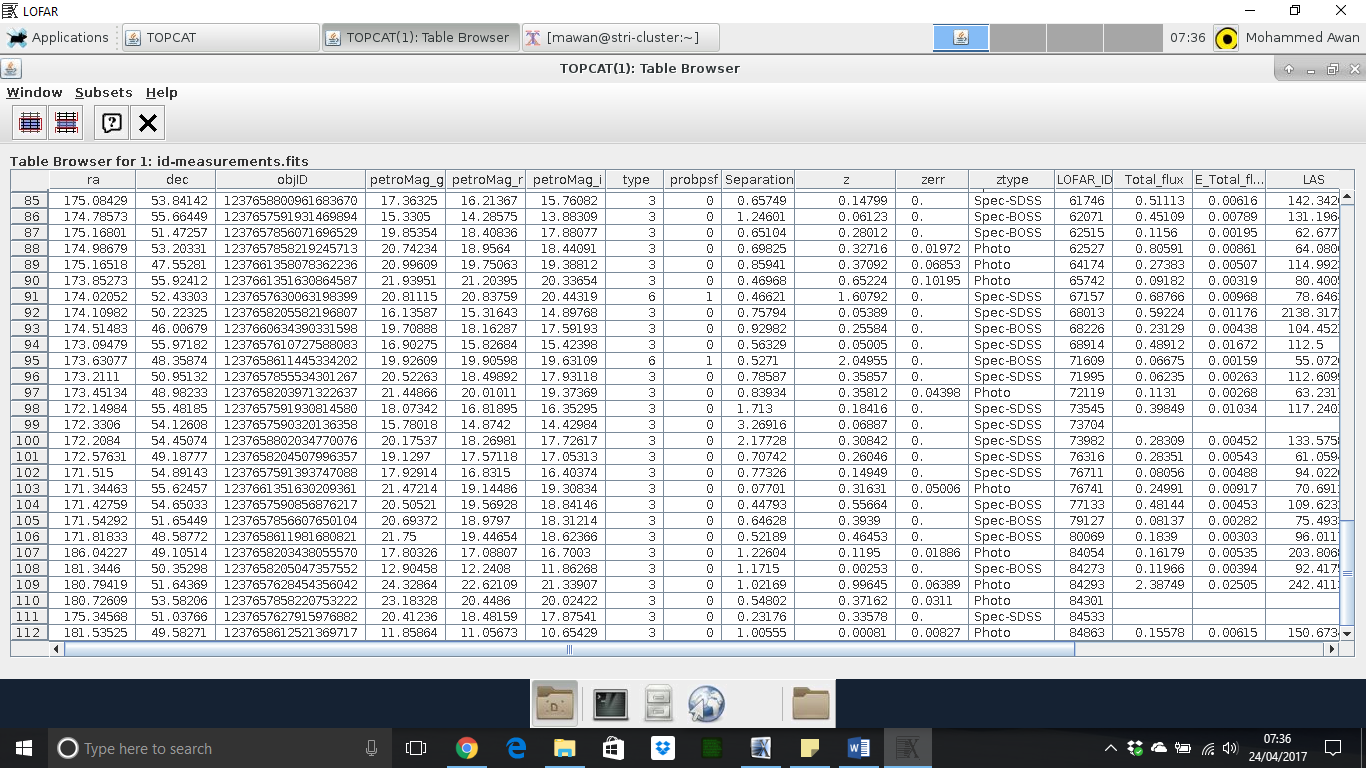
\includegraphics[scale = 0.4]{idmeasure.png}
    \caption{TOPCAT database output from id-measurement.fits file }
\end{figure}

The SDSS survey was then loaded (it was contained in a file called sdss-withz.fits). Note there are almost 3 million sources in this database!

\begin{figure}
    \centering
    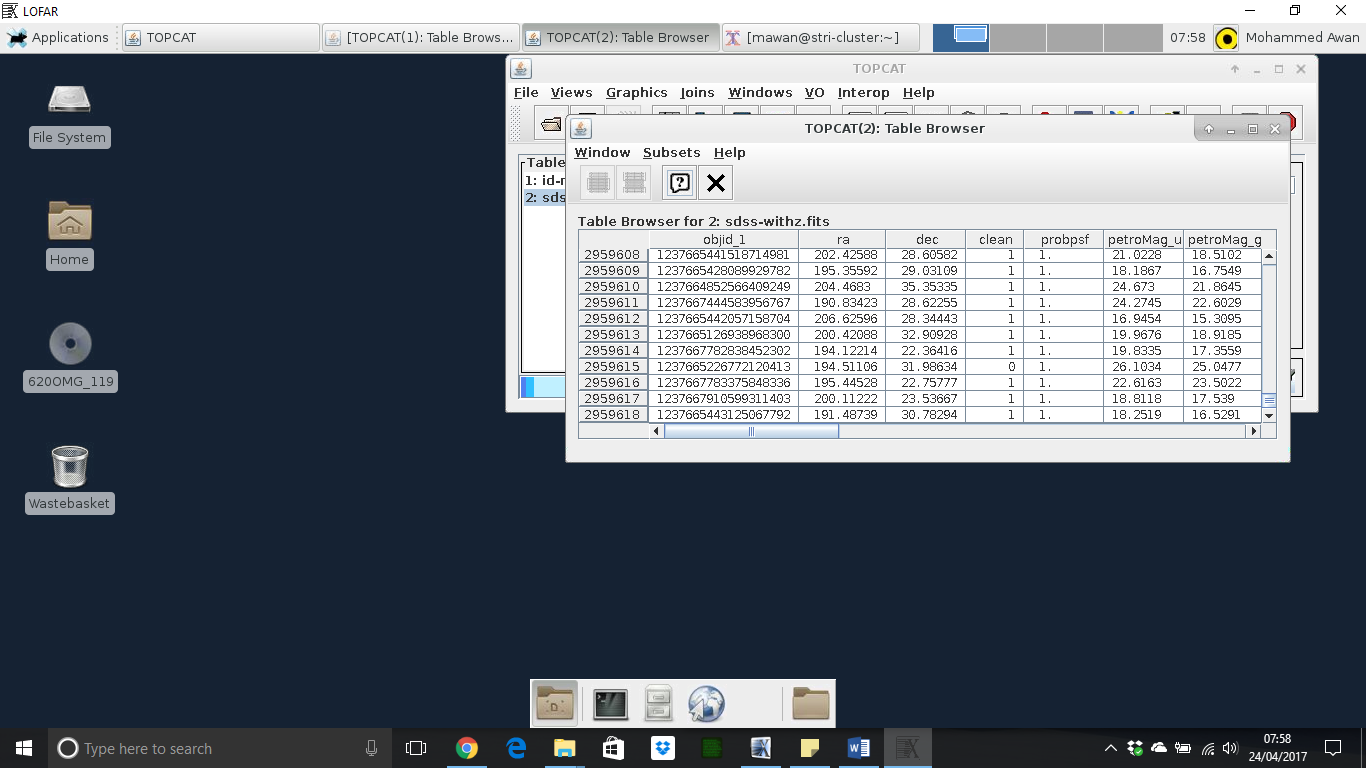
\includegraphics[scale = 0.4]{sdss.png}
    \caption{TOPCAT database output from SDSS}
\end{figure}

Included are individual normalised histograms for the z values of both the sample data and the sdss field as well as comparisons with the h-atlas survey. Analysis is included below the plots

\begin{figure}
    \centering
    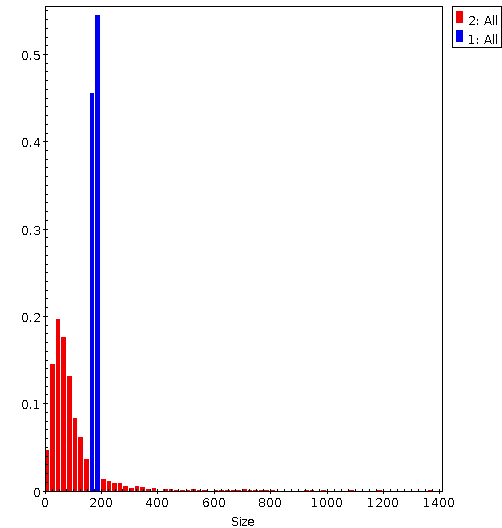
\includegraphics[scale = 0.4]{hatlassamplesize.png}
    \caption{Plot of normalised histograms of calculated samples:Note the blue distribution (sample) is clearly biased towards large sizes than the unsampled h-atlas data (red)}
\end{figure}


\begin{figure}
    \centering
    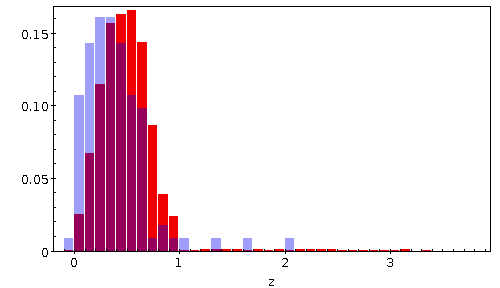
\includegraphics[scale = 0.4]{hatlasandsamplez.png}
    \caption{An overlay of the z values of hatlas (red) and sample (blue) show that the blue values are more likely to be smaller, which indicates the sample data is more likely to be bright than data sampled wihtout constraint.}
\end{figure}

\begin{figure}
    \centering
    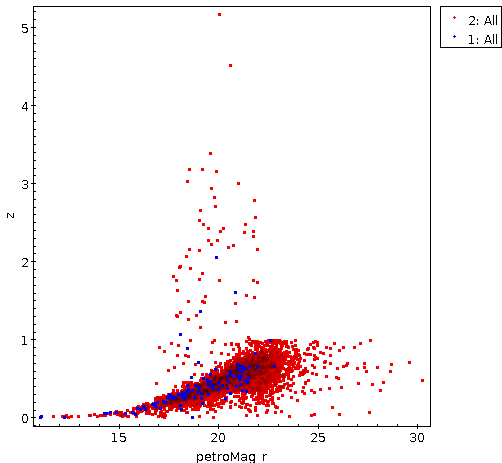
\includegraphics[scale = 0.4]{combihands.png}
    \caption{A scatter diagram of apparent magnitude versus z values for both sample (red and h-atlas (blue) data. It is difficult to draw any firm conclusions from this plot, however, the fact that the sample data seems to be a subset of the the larger h-atlas data set seems to add credence to the validity of both the data and the approach. It is possible that mean values for the sample z values and apparent brightness (which what petroMag r symbolises) seems to a most likely value in the region of 0.3 and 20 respectively. A closer examination of a magnified version of this plot would most likely make it more useful}.
\end{figure}

\begin{figure}
    \centering
    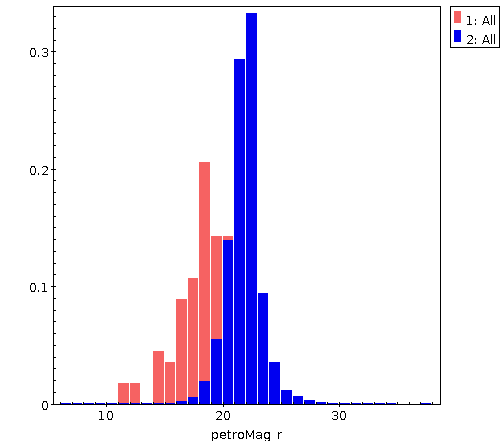
\includegraphics[scale = 0.4]{combip.png}
    \caption{The bias of the sample data (blue) as compared to the SDSS data (red) towards larger than average sizes is clearly discernible.}
\end{figure}

\begin{figure}
    \centering
    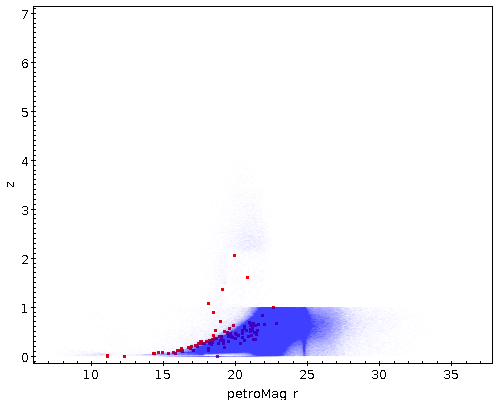
\includegraphics[scale = 0.4]{combizp.png}
    \caption{Although difficult to interpret. The distribution of the sample dots (red) as compared the translucent distribution of the nearly 3 million SDSS sources do not seem to indicate much, but the bias of bright, big sources is easily inferred from the figures above. To be more useful the sample size data would have to be much larger.}
\end{figure}


\subsection{Summary Remarks}

The analysis of the data in the plots below show that in comparison to the general surveys found in the SDSS and H-Atlas data, the sample data is clearly biased towards producing bright, large sources. While there are many plausible explanations of this effect the most logical seems to be that the data preferentially selects bright, old sources as these are the ones that are most readily detectable given our limits of precluding any sources less than 0.05 milli Janskis in apparent brightness and which are any smaller than 35 arc seconds in size.

\section{conclusion}
\subsection{summary of skills gains and results obtained}
In conclusion, the objectives of the project were largely met: a thorough understanding and introductory competency of using the various tools and environments necessary to conduct basic research in modern radio astronomy. A useful sample data set was extracted, optically identified and analysed. The main conclusion drawn on the type of data that selection criteria was biased towards selecting were, old bright sources, due to the relatively large values for apparent magnitude and size that were finally selected.

\subsection{Avenues for further investigation}
There are many further and exiting avenues for future investigation. The particular surveys utilised in this project are subject to intensive research at the time of writing by a number of professional scientists. If the research was continued at this stage, obvious next steps would be to:
\begin{itemize}
    \item develop a programme so that the process of selection could be automated. It is hoped that the sample selection could play a part in the machine learning process.
    \item A more thorough investigation into the physics properties of identified sources. As previously stated, the causes behind the emission of AGN jets is not yet fully understood and new data is being released on a regular basis. An initial step in this process would be to compare the sample images with more detailed optical images in hope of gaining further insight into their natures and possibly the mechanisms behind them.
    \item Use the tools developed in this project to study other phenomena which have active radio signatures.
\end{itemize}
\newpage

\bibliographystyle{unsrtnat.bst}
\bibliography{references}
\end{document}
